\chapter{結果統合}

\section{a}
% 有効な結果を示した
% kaldi
% 論文
% キャッシュモデル or N-gram特徴量
% 前後の部分文書の情報の加味
% を利用して最大値を試す

% TODO: 前章 = N章と名義した方が良い

前章で検索性能に有効な結果を示した,論文の利用・Kaldiを用いた検索文書の利用・キャッシュモデルとN-gram特徴量の加味・前後の部分文書の情報を加味の手法を統合し,更なる検索精度の改善を行う.

\subsection{実験条件}
実験条件を表\ref{t_ex_patern}に示す.

\begin{table}[h]
    \centering
    \caption{実験条件}
    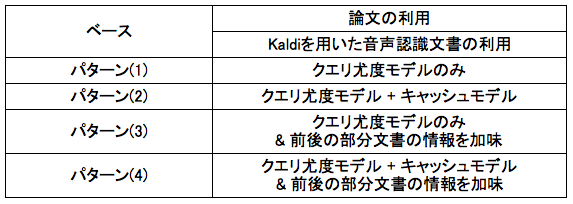
\includegraphics[width=7cm]{./image/t_ex_patern.png}
    \label{t_ex_patern}
\end{table}

基本的に論文の利用・Kaldiを用いた検索文書の利用・・前後の部分文書の情報を加味・クエリ尤度モデルを利用し,パターン1 クエリ尤度モデルのみ, パターン2 キャッシュモデル, パターン3 N-gramモデルを変化させたときのMAP値を算出し,分析する.また,パターン3のN-gramモデルのスムージングはKneser-Ney スムージングを利用し,N-gramのNは3とした.
